\documentclass[10pt, conference, compsocconf]{IEEEtran}

\usepackage{graphicx}
\usepackage[export]{adjustbox}
\usepackage{mathtools}
\DeclarePairedDelimiter\ceil{\lceil}{\rceil}

\begin{document}

\title{Build your own OctopusDB: Blinktopus Edition}
\author{ \\  \\ }

\author{\IEEEauthorblockN{Pavlo Shevchenko, Ali Hashaam, Guzel Mussilova, Ali Memon}
\IEEEauthorblockA{Otto-von-Guericke-University, Magdeburg\\
firstname.lastname@st.ovgu.de}}
%%\and\IEEEauthorblockN{Gabriel Campero Durand}\IEEEauthorblockA{Otto-von-Guericke-University, Magdeburg\\gabrielcampero@acm.org}}

\maketitle

\begin{abstract}
What is this paper about?
\end{abstract}
%%\section{Abstract}

\section{Introduction}
%%Motivation. Main Idea. Goal. Structure of the paper. Contribution.
%%\subsection{Background and Motivation}
Over the last decades we are witnessing that modern enterprises need to pick only  specialized DBMSs(e.g. OLAP, OLTP, streaming systems and etc.) each tailored to their specific use-case. Consequently, it leads to additional costs in terms of licensing, maintenance, integration and man-hours for DBAs. Although, it is affordable for some companies, to adapt these integrated solutions to constantly changing workloads and requirements, it may still be a challenging and non-trivial task to achieve. Thus, in order to cope with these problems an implementation of a new all-purpose system could be a perfect solution. 

Nowadays there exists a great variety of systems that claim to solve the aforementioned problems and yet their cost might be quite prohibitive. Some traditional DBMSs(e.g., Microsoft SQL Server, Oracle, ...) have already included the support of both analytical (OLAP, which is characterized by long-running queries over all the values of few columns) and transactional (OLTP, characterized by short-lived transactions that affect all attributes of few rows) workloads. Meanwhile, in the last 15 years these systems have been observed to be inefficient for new memory-rich architectures. As a consequence, exploiting the benefits from larger memory new DBMSs have been proposed, which have a simpler architecture than traditional disk-based ones and already proved to be more efficient than those. Among these recent solutions are the column-stores(e.g., C-Store[13], MonetDB[8], ...) and the row-stores(e.g., Hekaton[7], H-Store[14], MemSQL[15], ...) that are particularly designed for analytical and transactional processing, respectively. 

Still, following the \textit{one size does not fit all} observation these systems have mainly specialized either for OLAP or for OLTP[6]. Thus, it has lead the various vendors to try to build the comprehensive solutions, namely Hybrid Transactional/Analytical Processing (HTAP) systems(the term HTAP was defined by Gartner[17]). Some examples including SAP HANA[9] which has the engines that are optimized for OLAP workloads, at the same time it also supports ACID transactions. HyPer[10] is another example, which has a hybrid approach that uses memory snapshots based on process forking. Other examples include Peloton[11], OctopusDB[1] and  SnappyData[16] that also belong to HTAP systems.  \\
One of the solutions that most radically departs from existing architectures was proposed by Jens Dittrich and Alekh Jindal - a new type of database system, coined OctopusDB[1].
\begin{figure} 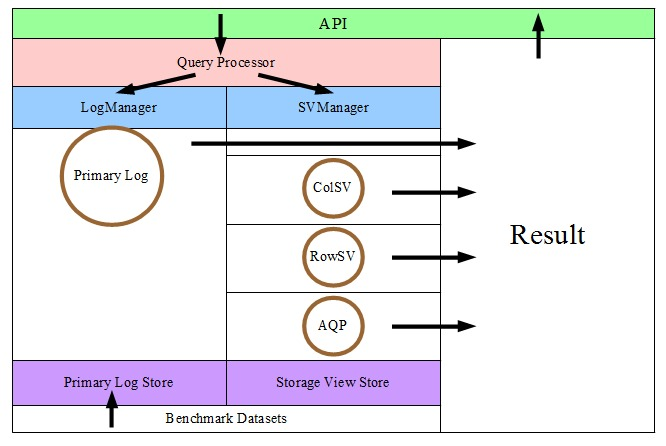
\includegraphics[width=0.4\textwidth, center]{img/blinktopus_architecture.jpeg} 
\caption{Blinktopus Architecture.}
\end{figure}
By dynamically mimicking several types of systems(OLAP, OLTP, Hybrid of OLAP and OLTP and etc.) and using logs as a primary storage, OctopusDB shows a considerably better performance. Moreover, depending on the use-case it may also emulate data stream management systems by replacing some of the stores with streaming windows. 

Another important goal of HTAP systems(aside from maintaining different system components compatible in order to create an illusion of a single system) is to support OLAP queries for analysis over real-time data. The fact that HTAP systems might reduce the need for transforming data from one system to another(via ETL), seems like a good step towards the support of real-time data. We believe that the exploration of the techniques related to more interactive queries, can contribute to the real-time characteristics of HTAP systems. Among the techniques that can handle more interactive queries Approximate Query Processing(AQP) have recently gained a substantial attention. By processing the compact synopsis of the data rather than the whole dataset, the methods for AQP are often the only viable solution to provide interactive response times when exploring massive datasets and handling high speed data streams[12]. Several successful examples(e.g. BlinkDB, SnappyData on Facebook's Presto) have already proved that there are benefits to be gained by integrating approximation features into existing DBMSs[5].\\
In this paper we want to evaluate the role that AQP can play as an architectural addition, in a HTAP system like Octopus DB, for facilitating real-time queries on the latest data. %%Meanwhile, it became evident that a system performance can be further enhanced by applying techniques from completely different perspectives. 
We believe that when it is plausible for a system to retrieve results approximately rather than exactly, AQP could be a reasonably good fit to further improve the performance of query processing (especially, OLAP queries). It could also enhance HTAP by answering the OLAP queries over new data that even has not been included yet and when it is guaranteed that a given amount of incoming data will not change the error of an estimation. Combining OctopusDB and AQP techniques could be feasibly good solution for improving HTAP \textit{freshness} and the performance of our system. In this paper we provide an early evaluation on these aspects.\\
%%Thus, our goal is to provide a user a tool called Blinktopus, that will allow  to build his own prototype of OctopusDB with embedded AQP techniques.

Our contributions are:
\begin{itemize}
\vspace{0.05 cm}
\item{We review the ideas of OctopusDB and AQP along with the concepts of AQP main data synopses(Section 2).}
\item{We propose a novel concept of a new system called Blinktopus and explain why exactly one type of AQP data synopsis was chosen for our system(Section 3).}
\item{We provide an experimental evaluation on the benefits of Blinktopus's functionality based on the results of the tests performed on the Storage Views(SVs) with the different physical layouts, namely LogSV, ColSV and RowSV(Section 4).}
\item{We discuss related work (Section 5) and future directions for our research(Section 6).}
\end{itemize}

\section{Fundamentals}
Firstly, we discuss the core idea of OctopusDB, its motivation and  architecture(Subsection A). Afterwards we explain the main concept of AQP and elaborate AQP main data synopses such as samples, histograms, sketches, wavelets and etc(Subsection B).
\subsection{OctopusDB}
%%As it was mentioned earlier, most companies currently have to manage how to keep the \textit{zoo} of systems, each designed for a specific use-case scenarios. Even though some enterprises that invest a lot might be able to afford the maintenance of different systems and/or by integrating they might eventually get a single all-embracing solution. Whereas it might be still beyond the strength of most small- and medium-sized companies. Moreover, systems that adhere the principles of traditional DBMSs might not be able to deliver the best performance or to fulfill some use-cases. Thus, the motivation to create new database system with \textit{one-size-fits-all} architecture which is suitable for different scenarios is quite eloquent. 
OctopusDB is one of the representatives of \textit{one-size-fits-all} architecture systems. %%The most striking difference of OctopusDB's architecture is that in comparison with other DBMSs it does not have a predefined fixed store. 
It builds upon 2 ideas:\\
- Logs as a primary structure (which is similar to Samza[18], and other streaming systems).\\
- A storage engine with a programmable interface that allows users to specify how data will look like (e.g., RodentStore[23]).\\
All data in OctopusDB is stored in the central log named \textit{primary log}. The data is being collected into the log through the creation of logical log-entries of the insert/update operations, each record is identified by internally unique log sequence number \textit{lsn}. OctopusDB exploits the write-ahead loging(WAL) protocol and stores the primary log on durable storage(HDD or SSD). Depending on the workload, a so-called Storage View (SV) can represent the entire central log or some of its parts in different physical layouts(e.g., row-store, column-store, PAX, index etc.). 
For instance, for OLTP queries OctopusDB can create Row SV, Col SV - for OLAP. Moreover,  it can optionally decide to create other materialized view such as Index SV or even to mimic streaming systems. At the same time, primary log is another SV for OctopusDB.  

Another component of Octopus DB called \textit{Holistic Storage View Optimizer} solves a non-trivial optimization task of \textit{storage view selection}(i.e., to determine automatically which type of SV is proper to be created). It maintains all SVs including primary log as well as it is responsible for creation and maintenance of secondary SVs. By means of scanning the indices and whole tables, later  depending on cost model the optimizer resolves either to create new SV or to maintain an existing one or even to scan the log when none of SVs can answer the query. Furthermore, by applying a transformation cost model it might transform different SVs one into another. Additionally, it can remove from system all SVs. Thus, based on the workload and arbitrary occurring use-cases the holistic SV optimizer operates a \textit{storage view lattice}(i.e., the dependency graph between SVs), within the Storage View Store of the OctopusDB.

OctopusDB can be recovered by easily copying the primary log from durable storage to main memory. Meanwhile all SVs that were in the OctopusDB before the system crash will be re-created.

Furthermore, OctopusDB supports ACID. For instance, \textit{Consistency} can be ensured by validating the set of integrity constraints at commit time and \textit{Durability} holds because OctopusDB keeps WAL. The \textit{Isolation} algorithm of OctopusDB is represented via optimistic concurrency control. Whose basic concept is to store all committed or uncommitted changes in the primary log and to write only committed data in secondary SVs. Committed data is available for \textit{read} by uncommitted transactions from log or any secondary SV. Moreover, the latter modifications are possible by adding records to the log but these data will not be further propagated to the secondary SVs for a while. To that end, \textit{Atomicity} is guaranteed by storing in SVs only committed transactions for their latter considerations by other transactions.

\subsection{Approximate Query Processing}

%%Main Idea. Synopses for Massive Data: Histograms. Sketches.More on histograms. Probably something on HLL, if it's eventually included in Blinktopus.

It is already evident that nowadays an enormous amount of data is being generated, processed and stored. Even the fastest systems can get stuck for hours in answering simple queries and this response time is less than satisfactory for users and applications. At the same time, in many cases(e.g., a/b testing, exploratory analytics, big data visualization and etc) providing the exact answers to a user query is not vitally important as long as estimations can result in the right decisions. AQP methods can achieve interactive response times(e.g., sub-second latencies) over a massive amount of data by processing only small fraction of the relevant records. 

AQP systems differ according to their methodology and design options. AQP operates the datasets through its predefined types of summaries(e.g., \textit{samples, histograms, wavelets, sketches} and so on) that capture main features of initial data while using less space. Such aspects as accuracy, range of applicability, space and time efficiency, error bounds on approximate answers strongly depend upon the chosen types of data synopses and their parameters. In addition, another issues in terms of data summaries(i.e., offline or online data summarization, various storage and maintenance strategies and etc) also need to be taken care of.

\textbf{Samples} perhaps are the most researched and extensively implemented type of data summaries. Their prevalence was induced by many reasons. As one the oldest concepts in statistics, there exists a great variety of schemes to extract and maintain samples of data varying in precision and accuracy, such as \textit{Bernoulli sampling, stratified sampling, random sampling with and without replacement} and others. \\
By using the same schema as the original relation, most queries can be performed over a sample(i.e. small "representative" subset of data) with slight or no alterations to existing system, so they can answer the widest range of queries. In spite that an immense diversity of queries can be evaluated using sampling methods, performing MIN, MAX, top-K and COUNT DISTINCT queries on a sample is quite impractical. At the same time, by avoiding \textit{AVI(Attribute Value Independence)} assumption, most sampling algorithms might support high quality selectivity estimation[19].

Moreover, sampling-based approximations do not suffer from "curse of dimensionality", i.e., their accuracy does not deteriorate with the increasing number of data dimensions. However, some samples are not suitable for handling outliers in skewed distributions. 

Finally, adding the estimation from several samples can incrementally enhance an imprecise estimate of a query result in interactive exploration of large dataset in "Online aggregation" algorithms. Notwithstanding, when the data is constantly updated in the massive data streams and the majority of future queries are not known in advance, it is crucial to make certain of samples being kept optimal and up to date. 

\textbf{Wavelets} are another means of data synopses utilized by AQP systems over large datasets. The core idea of wavelet-based approximations is to transform the input relation in order to acquire a compact data summary that will consist of a small set of wavelet weights or coefficients. While by capturing significant features of the massive dataset wavelets can ensure substantial data compression, they as histograms have the same "curse of dimensionality" limitation. Though this issue can be tackled by efficiently built wavelet decomposition, most implementations revolve around the one-dimensional cases, which can answer a limited spectrum of queries. Moreover, the error guarantees provided by wavelets seem not to be always meaningful in the context of AQP[22]. Still an appropriately-defined AQP algebra, which manages the domain of wavelet coefficients, assures answering range and more general SPJ(select, project, join) queries. 

As an example of the wavelet synopsis \textit{Haar Wavelet Transform(HWT)} is probably conceptually the easiest and therefore the most widely implemented wavelet transformation. Based on recursive pairwise averaging and differencing the resulting wavelets are straightforwardly computed and have been observed to show practically acceptable performance for numerous number of applications(e.g., image editing, querying to OLAP and streaming-data).\\

\textbf{Histograms} are another type of data synopses for summarizing the frequency distribution of an attribute or sets of attributes. Basically, a histogram groups input data values into subsets(i.e., "buckets", "bins") for each bucket it computes a small summary statistics in order to use it further for approximate reconstruction of the data in the bucket. In designing histograms the following aspects are to be carefully considered.  \\
- \textit{Bucketing scheme}. Data items must be distributed within the buckets in order to better represent its structure. It can be decided depending on some local criteria(e.g., value frequencies or similarities etc.) or some global "optimality" criteria of the histogram according to a workload or a query class.\\
- \textit{Intra-bucket approximation scheme}. In essence, there have been used two methods(e.g.,\textit{continuous value assumption} approach and  approach of \textit{uniform spread assumption}[24]) for intra-bucket approximation scheme of one-dimensional histogram. Both of them assume that values are uniformly distributed within the bucket range, with the first neglecting the number of the values and the second storing that number in the bucket. For the multi-dimensional histograms these approaches are to be extended. The choice of approximation scheme can also depend on the class of queries that histograms answer.\\
- \textit{Statistics stored per bucket} can contain the number of items in each bucket along with the subset boundaries. The method chosen for the data approximation usually defines what information will be stored.\\
- \textit{Bucket width}. The representation of real data via histograms may involve a loss of information, especially depending on the wrongly defined bucket width. Sturges's rule[30] is one of the commonly used rules. Moreover, other rules have been suggested that try to improve its performance without a normality assumption such as Doane's formula[29] and the Rice rule[28].\\ 
- \textit{Class of queries answered}. Even though histograms can answer a wide spectrum of queries(e.g., queries related to "selectivity estimation", range-count queries etc.), class of queries answered still needs to be carefully considered while building a histogram.\\ 
- \textit{Efficiency}. The cost of utilizing the histogram to provide query approximations, together with the time and space requirements can define the histogram from its efficiency perspective.\\
- \textit{Accuracy} in answering queries to a given size constraint is one of the most significant aspects when constructing an "optimal" histogram. \\
- \textit{Error estimates}. Many histogram construction approaches claim to provide some "average" or "maximum" error estimates over a set of queries, which however might not hold for a specific query, or even class of queries. As long as histograms answer queries approximately, it is a question of demand to determine exact error boundaries possible for an each query issued. At the same time, mostly when these error estimates are provided, there is no other details on the errors. Hence, some works propose to store the maximum difference between the actual and the approximate frequency of a value within the bucket and by exploiting that to provide upper bounds on the error estimates produced by the histogram for range and other queries.\\
- \textit{Incremental maintenance}. This aspect is particularly significant when the values in the dataset are constantly and rapidly updated.
%%\textit{Partition rule} contains: \\
%%- \textit{Partition class} displays whether any restrictions on the buckets exist. For a serial class depending on some parameter(the next characteristic) the buckets are needed to be non-overlapping, while end-biased subclass needs only one non-singleton bucket. \\
%%- \textit{Sort parameter} is a parameter whose value for every element in the data distribution is obtained from the corresponding attribute value and frequencies. Attribute value(\textit{V}), frequency (\textit{F}) and area (\textit{A}) are some examples of sort parameters.\\
%%- \textit{Source parameter} uses the property of the data distribution and along with the next characteristic identifies a unique partitioning. Spread(\textit{S}), frequency (\textit{F}) and area (\textit{A}) are the most widely exploited source parameters. \\
%%- \textit{Partition constraint} is used as a mathematical constraint for a source parameter which solely determines a single histogram within its partition class. There have been defined few partition constraints such as equi-sum, v-optimal, max-diff and compressed.\\
%%\textit{Construction algorithm} builds histograms in compliance with the provided partition rule. Sometimes for the same class histogram there might exist several construction algorithms which differ in efficiency. \\
%%Independently of the histogram partition rule \textit{value approximation} shows how attribute values are approximated in the bucket. The continuous value assumption and uniform spread assumption imply that the values are uniformly spread within the certain range in the bucket.\\
%%\textit{Frequency approximation} indicates how frequencies are approximated within the bucket range. The uniform distribution assumption is the main method which assumes that all elements in the bucket are the same and equal to mean value of the actual frequencies.\\
%%Based on the information maintained in the histogram \textit{error guarantees} are the upper bounds on the errors of estimates generated by a histogram.

As a result of an active research in the area of histograms over the last decades, a great diversity of histograms schemes have been proposed. %They vary in the choice of the buckets, statistics stored per bucket, intra-bucket approximation scheme, classes of queries to be supported and how estimations are extracted. 
As long as they also barely support more than one data dimensions, one-dimensional histogram is the most preferable type. \\The simplicity in implementation and interpretation contributed to the popularity of \textit{equi-width} and \textit{equi-depth} histograms. Equi-width histograms do not overlap among the ranges of attribute values within the bucket and independent of their value frequencies have the same range size (or the number) of values in every bucket[21]. Since they store a greater amount of information than trivial ones, therefore often demonstrate better estimations. The reverse of equi-width histograms - equi-depth (or \textit{equi-height}) class of histograms has the same the sum of the frequencies of the attribute values with respect to each bucket, independent of the range size(i.e., the number) of these values. According to the studies of Piatetsky-Shapiro and Connell who also gave this class of histograms its name, equi-depth histograms have lower worst-case and average error values for a diverse set of selection queries than equi-width histograms.
Beyond aforementioned types, more others have been introduced such as \textit{serial}[21], \textit{end biased} and \textit{high biased}, \textit{maxdiff} and other generalizations. 

Another aspect which also worth taking into consideration is a construction cost. With regard to it, histograms can be divided into two groups: \textit{static} and \textit{dynamic} or \textit{adaptive} histograms[20]. Static histograms are commonly used in DBMSs. After they are built, even when the data is being changed, they remain unaltered. Hence, with the time a static histogram drifts away from its "up-to-date" state and its estimations may deteriorate from progressively larger errors. When this occurs, these histograms are recalculated and the old histograms are replaced with the "fresher" versions. 
Despite of the fact that there have been proposed some efficient calculation algorithms for static histograms, adaptive histograms are the only viable option in a data stream environment. The most known examples of dynamic histograms are \textit{equi-depth and compressed} histograms[25], \textit{v-optimal} and \textit{spline-based} histograms. 

Histograms efficiently answer range-sum queries and their variations. Furthermore, they can be utilized to approximate more general classes of queries(e.g., aggregations over joins), as well as real-valued data and set-valued queries.
  
As it is already known histograms are one of the most implemented data summaries. Since they can be incorporated into existing database system without obtaining an additional storage overhead, they are mainly exploited by query optimizers of almost all DBMSs to produce cost and selectivity estimations of various query plans. However, wrong estimations in query optimizers continue to be an important problem in database systems.

\textbf{Sketches} are especially germane for the streaming data, where the data in a large scale is being processed and the sketch synopsis must be updated promptly and effectively without exploiting huge compute resources. Sketching algorithms use hash functions with defined mathematical properties that provide their guarantees, but in practice these hash functions are rather simple and rapid, with reference implementations that are broadly available.  

Sketch summaries can be designed so that each new update will be independent of the latest state of synopsis. For instance, linear sketches consider a numerical dataset as a matrix or vector, and multiply the data by another fixed matrix. These types of sketches are easily parallelizable. Moreover, for the some queries(e.g., count distinct, most frequent items, joins, graph analysis and matrix computations), sketches may be the only viable solution.

"Frequency based sketches" summarize a dataset frequency distribution and provide accurate estimates of individual frequencies. This results in algorithms for calculating "heavy hitters" - items that account for a large portion of the frequency mass - and quantiles like median and its generalizations. These sketch summaries can similarly be utilized to approximate range queries, the sizes of (equi)joins between relations and self-join sizes. Moreover, such sketches may be exploited to extract histogram and wavelet representations of streaming data and as elements of more complex mining operations.

As was mentioned above sketch-based summaries are especially suitable for “distinct-value” queries(i.e., to count the number of distinct values in the dataset). Once built, these sketches approximately can estimate the cardinality of a given attribute or combination of different attributes. Furthermore, they can calculate the cardinality of various operations performed on them(e.g., selections based on arbitrary predicates along with the set operations such as union and difference). One of the most well-known examples of using sketches for DISTINCT COUNT queries is a near-optimal probabilistic algorithm of \textit{HyperLogLog}. 

HyperLogLog methodology has been successfully implemented by Yahoo and improved the performance of its internal platform from days to hours and somewhere even to minutes[26]. It exploits an auxiliary memory of \textit{m} units and by passing over the multiset once, estimates its cardinality with the standard error of nearly 1.04/$\sqrt{\textit{m}}$. For instance, while utilizing only 1.5 kilobytes of a memory, this algorithm is capable of estimating cardinalities beyond $10^9$ with a typical accuracy of 2\%[27].

Although, the sketching techniques can answer a considerable number of query types. However, they do not observed to scale well to more complex queries that imply sub-queries. Thus, the main drawback of sketches, especially in comparison with all-purpose sampling approaches, that they tend to answer a single type of query. 

Finally, the target workload defines which data summary to implement in the system. Most AQP systems that tailored for accelerating a diverse predefined set of queries, exploit sketches, wavelets and histograms, while sample-based approximations are usually used by all-purpose AQP systems. As a rule of thumb, AQP systems that combine several data synopses seem to demonstrate considerably efficient performance. 

\section{Blinktopus}
In this section we introduce a novel concept of our system called Blinktopus and give an explanation for the chosen type AQP data synopsis implemented in Blinktopus.  

\subsection{Architecture}

The core idea of Blinktopus derives from two cornerstones:\\
1. Blinktopus is an adaptive system that according to user command mimicks different types of systems(e.g., OLAP, OLTP) and as an output provides an SV which answers user queries.\\
2. Since AQP techniques guarantee better interactive response times to a user query(especially, OLAP queries) over the "fresher" data, Blinktopus uses AQP techniques to further enhance its performance.

In the Fig. 1 we present the architecture of Blinktopus. Similarly to Octopus, Blinktopus also does not have a fixed store and all data is stored in a \textit{primary storage} or \textit{primary log}.
All data from the log or its some parts is represented via materialized SV namely \textit{LogSV}, which is as another type of SV can be used for answering the queries. The component of \textit{LogManager} defines the structure of LogSV and operates it within a \textit{Primary Log Store}. 

In general, besides LogSV, Blinktopus can manipulate the dataset via other secondary types of storage views: column SV(\textit{ColSV}), row SV(\textit{RowSV}) and AQP SV(\textit{AQPSV}). Although, the latter is rather different from the first two, Blinktopus still considers it as another storage view over the data. This simplifies the implementation and allows further views to be added. Along with the data, relevant to the query, such views contain other information like the number of entries or the range of a data. 
%%However, the entries in our primary storage are different from the ones stored in LogSV. In OctopusDB, LogSV also contained the user's query which could be used for reconstruction purposes. In our cases, only the data is stored in the Log. 
%%The information about the views created needs to be stored in some predefined structure. 

Once created, the views can be accessed via \textit{SVManager}. This component is responsible for storing the views in the \textit{Storage View Store} and it also allows a user to get one or all of them and/or to remove them.
In spite the above-mentioned views can serve as the data storages, Blinktopus uses them only to provide the results to the user query. 

Finally, the central component that connects all the components of Blinktopus together is \textit{QueryProcessor}. It analyzes the query issued by a user and redirects it to the component which responsible for it.

Since Blinktopus answers only range queries and histograms are especially suitable for this class of queries and also due to their simplicity in implementaion and interpretation, together with acceptable error estimates we have chosen equi-depth type of histograms for AQP module of Blinktopus. They were constructed on the column of \textit{extendedprice} from \textit{LineItem} relation and \textit{totalprice} from \textit{Orders} on the whole dataset for COUNT queries.

The first step in constructing histograms is to sort the data with the attribute used(i.e., totalprice from Orders, extendedprice from LineItem). After the sorting, in order to calculate the number of buckets \textit{k} we used the simplified and enhanced version of Sturge's Rule - \textit{Rice Rule}.
\begin{equation}
k=\ceil*{2n^{1/3}}
\end{equation}

where \textit{n} - the number of elements in the dataset.
 
Since \textit{k} is determined, next step is to define the statistics stored per bucket. As long as AQP component of Blinktopus supports only COUNT queries, we decided to store the number of elements with its lower boundaries per bin, along with the highest boundary for the far rightmost bucket.

The front end part of Blinktopus is a user-friendly interface that facilitates user to act as \textit{Holistic SV Optimizer} in OctopusDB, i.e., to decide which of RowSV or ColSV to create/delete, or to which SV(e.g., RowSV, ColSV, LogSV or AQPSV) to address his query. 

Likewise, via this interface user is provided with opportunities to list all SVs created earlier in tabular or JSON format and delete all existing SVs.
The front end and back end parts of Blinktopus communicate via JSON files. After receiving and interpreting JSON files from back end side, front end provides user the results in the tabular format. Additionally, along with the query results, it visualizes in the form of bar charts the pre-calculated by back end query statistics(i.e., query runtimes and a comparison of the results performed over the different SVs).

\subsection{Workflow}

In this subsection we describe the workflow of user query processing in Blinktopus.
\begin{itemize}
\item{After query was issued, QueryProcessor interprets it. The query contains the table, column and a range of interest, as well as the SV type that user wants to use for the given query. In contrast to OctopusDB, where the Holistic SV Optimizer decided which SV to provide/create, in Blinktopus, this decision is made by user himself. However, a similar component that automatically will decide upon what storage view on a given query to provide can be easily implemented in the Blinktopus system.}
\item{After the query had been analyzed, QueryProcessor redirects it whether to the SVManager, if the specified view is either Column, Row or AQP module, or to the LogManager.}
\item{If user had chosen to look up over the log, then the whole primary storage will be scanned and the relevant tuples along with the information about the query (e.g. the table, the attribute, the range as well as query processing time) will be retrieved.}
\item{If any other type of secondary SV was chosen, depending on the user's choice, the SVManager will either invoke the creation of the specified view or retrieve the required data from already existing SV.}
\item{If user had chosen to query over the AQPSV, the function \textit{queryHistograms} sums up the number of elements for every bin that lie exactly within a given range. For the histograms buckets whose ranges were not covered completely within the bins, in order to provide an approximate result we use \textit{continuous value assumption}.}
\item{As it is not desirable for SVManager in order to retrieve the relevant tuples to scan the data, therefore SVs themselves are responsible for the result further retrieval and representation. Now when the view is created for the first time, the primary storage will be scanned and the relevant tuples will be formatted to fit to the desired view. Otherwise, an SV itself will scan the data it already stores and return to a user the only existing subset of the data.}

\end{itemize}

\section{Experimental Part}

Used dataset.

Evaluation of the test results:
 
1. Comparison of runtimes of different types of SVs.
2. Comparison of the diff SVs by means of percentage representation.

\section{Related Work}
In this section we briefly discuss several prior works and describe similarities and dissimilarities that they share with Blinktopus.

\textbf{Logs as a primary structure.} How the data is stored defines which data access techniques to implement in order to obtain the best performance possible for a certain database system. Most of modern DBMSs prefer to use a single data storage layout. Although, relying on the initial goal of the system such single-layout systems may acquire an exceptional efficiency, none of these choices may be a universally perfect solution. As a result, the most architecturally different systems have implemented new types of data storage layouts(e.g., tiles, logs, PAXes etc). 

Log is most probably one of the simplest data structures for DBMS. In essence, by supporting an appending write and sequential read, logs may not even require additional access methods. Therefore these systems eventually may show a better performance. Samza[31], OctopusDB[1] are examples of the systems that exploit logs as their primary storage. Where Samza also supports a so-called \textit{log compaction mode}, in which older messages are garbage-collected[31]. Moreover, in contrast to OctopusDB and Blinktopus, in Samza these logs are also being replicated(i.e., more scalable).\\
\textbf{Rodent Store} is a declarative and adaptive system that provides DBAs a high-level interface to specify the data physical representation by means of \textit{storage algebra}23]. In particular, adiministrators declare how to group and order a logical schema into sets of columns, rows and/or arrays. \\
\textbf{HTAP+AQP=SnappyData}.\\


\section{Conclusions}
Sum up what happened and provide future work

\section*{Acknowledgement}
Thanks to Gabriel(DBSE). Also we would like to thank Jindal, Dittrich and Mozafari for their awesome ideas that really inspired this project.

\begin{thebibliography}{1}

\bibitem{octopus_architecture}
Dittrich, Jens, and Alekh Jindal. "Towards a One Size Fits All Database Architecture." CIDR. 2011.
\bibitem{octopusdb}
Jindal, Alekh. "OctopusDB: flexible and scalable storage management for arbitrary database engines." (2012).
\bibitem{mimicking_octopus}
Jindal, Alekh. "The mimicking octopus: Towards a one-size-fits-all database architecture." VLDB PhD Workshop. 2010.
\bibitem{aqp_engines}
Mozafari, Barzan. "Approximate query engines: Commercial challenges and research opportunities." SIGMOD, 2017.
\bibitem{aqp_handbook}
Mozafari, Barzan, and Ning Niu. "A Handbook for Building an Approximate Query Engine." IEEE Data Eng.
Bull. 38, no. 3 (2015): 3-29.
\bibitem{one_size_does_not_fit_all}
M. Stonebraker and U. Cetintemel. "One Size Fits All": An Idea Whose Time Has Come and Gone. In ICDE, pages 2–11, 2005.
\bibitem{hekaton}
C. Diaconu, C. Freedman, E. Ismert, P.-˚A. Larson, P. Mittal, R. Stonecipher, N. Verma, and M. Zwilling. Hekaton: SQL Server’s memory-optimized OLTP engine. In SIGMOD, pages 1243–1254, 2013.
\bibitem{monetdb}
P. Boncz, M. Zukowski, and N. Nes. MonetDB/X100: Hyper-Pipelining Query Execution. In CIDR, 2005.
\bibitem{saphana}
F. Färber, N. May, W. Lehner, P. Große, I. Müller, H. Rauhe, and J. Dees. The SAP HANA Database – An Architecture Overview. IEEE DEBull 35(1):28–33, 2012.
\bibitem{hyper}
A. Kemper and T. Neumann. HyPer – A Hybrid OLTP'\&'OLAP Main Memory Database System Based on Virtual Memory Snapshots. In ICDE, pages 195–206, 2011.
\bibitem{peloton}
A. Pavlo, J. Arulraj, L. Ma, P. Menon, T. C. Mowry, M. Perron, A. Tomasic, D. V. Aken, Z. Wang, and T. Zhang. Self-Driving Database Management Systems. In CIDR, 2017.
\bibitem{cormode}
Cormode, Graham, Minos Garofalakis, Peter J. Haas, and Chris Jermaine. "Synopses for massive data: Samples, histograms, wavelets, sketches." Foundations and Trends in Databases 4, no. 1–3 (2012): 1-294.
\bibitem{c_store}
Mike Stonebraker, Daniel Abadi, Adam Batkin, Xuedong Chen, Mitch Cherniack, Miguel Ferreira, Edmond Lau, Amerson Lin, Sam Madden, Elizabeth O'Neil, Pat O'Neil, Alex Rasin, Nga Tran and Stan Zdonik. "C-Store: A Column-oriented DBMS." VLDB, pages 553-564, 2005. 
\bibitem{h_store}
H-Store. http://hstore.cs.brown.edu/
\bibitem{memsql}
MemSQL. http://www.memsql.com/
\bibitem{snappy}
SnappyData. https://www.snappydata.io/
\bibitem{gardner}
https://www.gartner.com/doc/3179439/predicts--inmemory-computingenabled-hybrid
\bibitem{samza}
https://www.confluent.io/blog/turning-the-database-inside-out-with-apache-samza/
\bibitem{babcock}
B. Babcock and S. Chaudhuri. Towards a robust query optimizer: A principled and practical approach. In SIGMOD, 2005.
\bibitem{histogram_history}
Y. E. Ioannidis, “The history of histograms (abridged),” in Proceedings of the International Conference on Very Large Data Bases, pp. 19–30, 2003.
\bibitem{histogram_based_solutions}
Y. E. Ioannidis, V. Poosala, "Histogram-Based Solutions to
Diverse Database Estimation Problems." IEEE Data Eng. Bull. 18 (1995) 10-18.
\bibitem{wavelets}
S. Guha and B. Harb. Wavelet synopsis for data streams: minimizing non-euclidean error. In KDD, 2005.
\bibitem{rodentstore}
Philippe Cudré-Mauroux, Eugene Wu, and Samuel Madden. “The Case for RodentStore: An Adaptive, Declarative Storage System.” In CIDR. www.cidrdb.org, 2009.
\bibitem{improved_histogram_ioannidis}
Poosala V., Ioannidis Y., Haas P., Shekita E.: Improved Histograms for Selectivity Estimation of Range Predicates. SIGMOD Conf. (1996) 294-305
\bibitem{equi-depth_compressed}
Gibbons P., Matias Y., Poosala V.: Fast Incremental Maintenance of Approximate Histograms. VLDB Conf. (1997) 466-475
\bibitem{yahoo}
https://yahooeng.tumblr.com/post/135390948446/data-sketches
\bibitem{hyperloglog}
P. Flajolet, \`{E}ric Fusy, O. Gandouet, and et al., Hyperloglog: The analysis of a near-optimal cardinality estimation algorithm," in IN AOFA '07: PROCEEDINGS OF THE 2007 INTERNATIONAL CONFERENCE ON ANALYSIS OF ALGORITHMS, 2007.
\bibitem{bucket_width_rice_rule}
Lane, D.M.: Online statistics education: an interactive multimedia course of study (2015). http://onlinestatbook.com/2/graphing distributions/histograms.html. Accessed 03 Dec 2015
\bibitem{doane_formula}
Doane, D.P.: Aesthetic frequency classifications. Am. Stat. 30(4), 181–183 (1976)
\bibitem{sturges_rule}
Hyndman, R.J.: The problem with sturges rule for constructing histograms. Monash University (1995)
\bibitem{samza_kafka}
Kleppmann M., Kreps J.: Kafka, Samza and the Unix philosophy of distributed data. IEEE Data Engineering Bulletin 38(4):4–14, December 2015.
\end{thebibliography}

\end{document}\grid
